\vspace{0.5cm}
In the Deployment diagram in the figure are shown the most important components.
\vspace{1cm}
\begin{figure}[H]
  \centering
  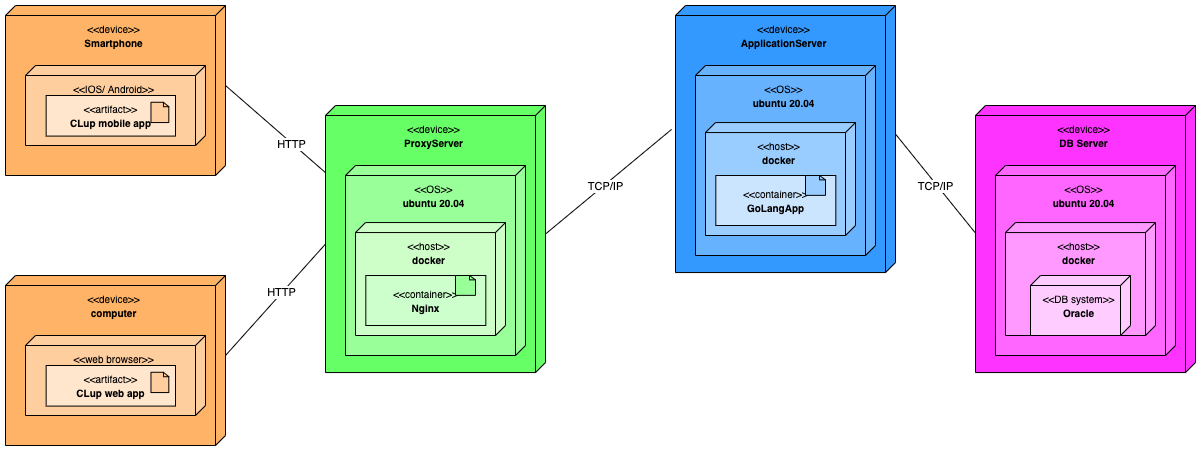
\includegraphics[width=\textwidth, keepaspectratio] {images/all/deploymentview.png}
  \caption{Deployment Diagram}
\end{figure}
\vspace{2cm}

The deployment has some devices: \\
\begin{itemize}
    \item \textbf{Smartphone:}  the user will use, which can be a smartphone or a tablet using as operating system either iOS or Android. The execution environment is the built CLup app.\\
    
    \item \textbf{Computer:} the clerk use this to put the offline user in the line and it also has scanner to scan user ticket in entrance and checkout from the shop.\\
    
    \item \textbf{Proxy Server:} in this device we use nginx as a reverse proxy server. A reverse proxy accepts a request from a client, forwards it to a server that can fulfill it, and returns the server's response to the client. \\
    
    \item \textbf{Application Server:} It is supposed to be a dedicated server running a linux distribution specific for server use. As an example of OS we choose Ubuntu. Other distribution can be used like Red Hat Enterprise Linux, Debian, OpenSUSE. As execution environment we use GoLanng because it is fast and suitable for microservice.\\
    
    \item \textbf{DB Server:} It consists in another server where we run the DB system Oracle. We choose to run the database in a separate server and not in the same as the Application Server in order to increase scalability. 
\end{itemize}
As you can see in the diagram, we install docker in all of our server to increase portability and easy deployment of the servers.
